%Pavel Chvykov


% ***********************************************************
% ******************* MY HEADER ************************
% ***********************************************************
%\documentclass[11pt]{article}
\documentclass[reprint,prx]{revtex4-1}
%\documentclass[twocolumn,showpacs,preprintnumbers,amsmath,amssymb,superscriptaddress]{revtex4-1}
%\usepackage[greek, english]{babel}

\usepackage{amsmath} % AMS Math Package
\usepackage{amsthm} % Theorem Formatting
\usepackage{amssymb}	% Math symbols such as \mathbb
\usepackage[pdftex]{graphicx}
\usepackage{epstopdf}
\usepackage{enumerate}
%\usepackage{multicol} % Allows for multiple columns
\usepackage{wrapfig}
\usepackage[dvips,letterpaper,margin=1in,bottom=1in]{geometry}
\usepackage{color}
%for writing tensors (syntax: `G_ab^gl_d`)
\usepackage{tensind}
\tensordelimiter{`}
\whenindex{a}{\alpha}{} \whenindex{b}{\beta}{} \whenindex{g}{\gamma}{} \whenindex{d}{\delta}{} \whenindex{e}{\varepsilon}{} \whenindex{m}{\mu}{} \whenindex{n}{\nu}{} \whenindex{l}{\lambda}{} \whenindex{k}{\kappa}{} \whenindex{r}{\rho}{} \whenindex{s}{\sigma}{} \whenindex{t}{\tau}{}
\usepackage{todonotes}
\usepackage{subcaption}
% % Sets margins and page size
%\pagestyle{empty} % Removes page numbers
\usepackage{setspace}
%\onehalfspacing
%\setstretch{1.1}
\usepackage{comment}
\usepackage{cancel}
%\usepackage{xfrac}
\usepackage[]{units}

\usepackage{hyperref}
\usepackage[all]{hypcap}
%\usepackage[toc]{appendix}

\makeatletter % Need for anything that contains an @ command 

%\renewcommand{\maketitle} % Redefine maketitle to conserve space
%{ \begingroup \vskip 10pt \begin{center} \Large {\bf \@title}
%		\vskip 10pt \large \@author \\ \@date \end{center}
%		\vskip 10pt \endgroup \setcounter{footnote}{0} }


%\makeatother % End of region containing @ commands
%\renewcommand{\labelenumi}{(\alph{enumi})} % Use letters for enumerate
% \DeclareMathOperator{\Sample}{Sample}
\let\vaccent=\v % rename builtin command \v{} to \vaccent{}
\renewcommand{\v}[1]{\ensuremath{\vec{#1}}} % for vectors
\newcommand{\gv}[1]{\ensuremath{\mbox{\boldmath$ #1 $}}} 
% for vectors of Greek letters
\newcommand{\uv}[1]{\ensuremath{\mathbf{\hat{#1}}}} % for unit vector
\newcommand{\abs}[1]{\left| #1 \right|} % for absolute value
\newcommand{\avg}[1]{\left< #1 \right>} % for average
\let\underdot=\d % rename builtin command \d{} to \underdot{}
\renewcommand{\d}[2]{\frac{d #1}{d #2}} % for derivatives
\newcommand{\dd}[2]{\frac{d^2 #1}{d #2^2}} % for double derivatives
\newcommand{\pd}[2]{\frac{\partial #1}{\partial #2}} 
% for partial derivatives
\newcommand{\pdd}[2]{\frac{\partial^2 #1}{\partial #2^2}} 
% for double partial derivatives
\newcommand{\pdc}[3]{\left( \frac{\partial #1}{\partial #2}
	\right)_{#3}} % for thermodynamic partial derivatives
\newcommand{\fd}[2]{\frac{\delta #1}{\delta #2}} %functional derivative
\newcommand{\fdd}[3]{\frac{\delta^2 #1}{\delta #2 \delta #3}} %second functional derivative
\newcommand{\ket}[1]{\left| #1 \right>} % for Dirac bras
\newcommand{\bra}[1]{\left< #1 \right|} % for Dirac kets
\newcommand{\braket}[2]{\left< #1 \vphantom{#2} \right|
	\left. #2 \vphantom{#1} \right>} % for Dirac brackets
\newcommand{\matrixel}[3]{\left< #1 \vphantom{#2#3} \right|
	#2 \left| #3 \vphantom{#1#2} \right>} % for Dirac matrix elements
\newcommand{\grad}{\nabla} % for gradient
\let\divsymb=\div % rename builtin command \div to \divsymb
\renewcommand{\div}[1]{\gv{\nabla} \cdot #1} % for divergence
\newcommand{\curl}[1]{\gv{\nabla} \times #1} % for curl
\newcommand{\tr}{\mbox{Tr}}
\let\baraccent=\= % rename builtin command \= to \baraccent
\renewcommand{\=}[1]{\stackrel{#1}{=}} % for putting numbers above =
\renewcommand{\deg}{^{\circ}} %degree simbol
\renewcommand{\(}{\left (}
\renewcommand{\)}{\right  )}
\renewcommand{\[}{\left [}
\renewcommand{\]}{\right ]}
\newcommand{\<}{\left <}
\renewcommand{\>}{\right >}
%\renewcommand{\{}{\left\{ }
%\renewcommand{\}}{\right\}}

\newtheorem{prop}{Proposition}
\newtheorem{thm}{Theorem}[section]
\newtheorem{lem}[thm]{Lemma}
\theoremstyle{definition}
\newtheorem{dfn}{Definition}
\theoremstyle{remark}
\newtheorem*{rmk}{Remark}
\newtheorem{?}{\textbf{Question}}

\newcommand{\e}[1]{\mbox{e}^{#1}} %exponential
\renewcommand{\exp}[1]{\mbox{exp}\[#1\]} %exponential
\newcommand{\intmom}[2][4]{\int \frac{d^{#1} #2}{(2\pi)^{#1}}} % 4D momentum integral
\newcommand{\intfn}{\int \mathcal{D}} %functional integral
\newcommand{\D}{\mathcal{D}}
\newcommand{\Ord}[1]{O\[#1\]}  %order of (big O notation)
\newcommand{\Op}{\mathcal{O}}  %operator
\newcommand{\im}{i}  %imaginary
\renewcommand{\todo}[1]{\textit{\color{red}[#1]}}
\newcommand{\um}{$ \mathrm{\mu} $m}
\renewcommand{\inf}{\infty}
\newcommand{\with}{\quad \text{with} \quad}
\newcommand{\at}[1]{\,\big |_{#1}} %evaluate at value
% ***********************************************************
% ********************** END HEADER *************************
% ***********************************************************

\begin{document}
\title{Predicting collective Smarticle motion}

\author{Pavel Chvykov}
\email{pchvykov@mit.edu}
%\affiliation{Physics of Living Systems, Massachusetts Institute of Technology} 
\author{Will Savoie}
\author{Dan Goldman}
\author{Jeremy England}
%		\thanks{pchvykov@mit.edu}


\maketitle

\tableofcontents

\section{Experimental setup and observations}
In this research, we seek to discover principles by which to analyze and predict future motion of a collective by performing a type of unsupervised statistical analysis on a prior test trials. This method is adapted from a way to classify stereotyped behaviors in biological systems and has not previously been applied to collective systems to the best of the authors’ knowledge. We believe this study is useful for data heavy collective systems which may have motion too complex for analysis through classical means. 

For this research, we use a collective of “smarticles” (smart, active particles) as seen in figure 1, a robotic system developed in Daniel Goldman’s lab, as a model system to serve as a case study to prove our method. Each smarticle is a three-link  two degree of freedom robot capable of changing its shape. Each smarticle on its own is immotile. However, an enclosed ensemble of smarticles can self-propel by utilizing the interactions arising from shape modulation of smarticles and the boundary enclosing them. Moreover, despite the stochastic nature of the interactions between elements, there seem to be various “states” or long lasting periodic collisional cycles that tend to persist over a long period of time.

\begin{figure}
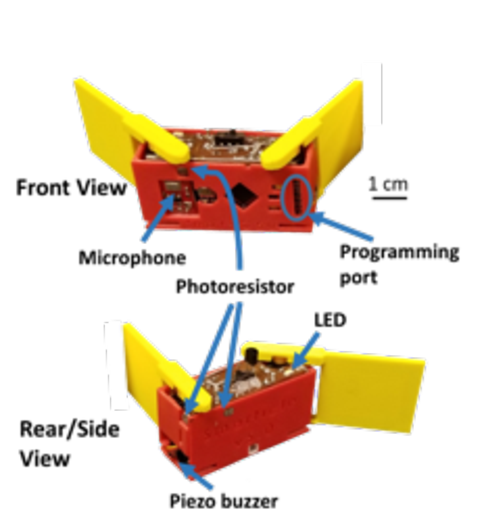
\includegraphics[width=0.3\textwidth]{Smarticle.pdf}
\caption{single smarticle with various sensors labelled}
\end{figure}

Previously we performed a study with smarticles where we tracked a ring containing 5 smarticles, travelling on a flat surface. The ring’s movement was a result of the collisions of the smarticles contained within it. Each smarticle continuously performed a square-gait, a periodic trajectory in the 2-degree of freedom configuration space of the smarticle centered around zero and shaped like a square. The trajectories of the ring, when analyzed seemed to have features of periodicity in them, see figure \ref{fig:run&tumb}. Upon further investigation, we found that these periodic trajectories, which tended to generate the largest amounts of movement of the ring, were a result of periodic collisional cycles in the ring. We believe that the very complex and stochastic motion of the ring could be characterized by the analysis of these periodic collisional states, or “regular states”.

\begin{figure}
	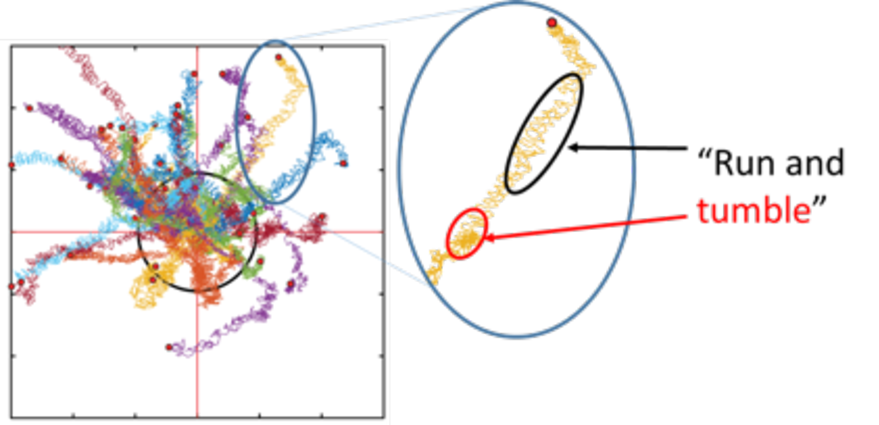
\includegraphics[width=0.45\textwidth]{RunTumbleRing.pdf}
	\caption{40 Supersmarticle trajectories, runs where highest displacement was achieved show high periodicity in the center of mass trajectory on short timescales. Black circle represents starting position of ring and is 19.2 cm \label{fig:run&tumb}}
\end{figure}

For the unsupervised regular state analysis, we simplified the system to aid in in the initial discovery of the regular states. We started with three smarticles, performing a continuous square gait completely in phase with their neighbors.

\begin{figure}
	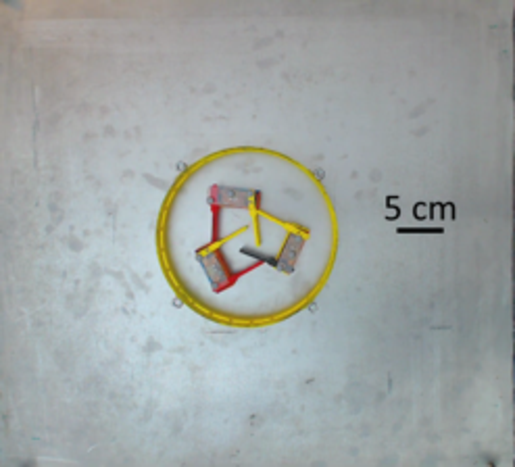
\includegraphics[width=0.3\textwidth]{3smRg.pdf}
	\caption{Regular state testing setup. The whole setup placed on an aluminum plate leveled to $ < 0.1\deg $. The ring is 19.2 cm in diameter, and is glued to the plate below such that it cannot move or deform. The smarticles perform a square gait locked in phase with each other.}
\end{figure}

\section{Identifying dynamical phases from data}

Once we have the tracked coordinates of the smarticles, we want to map the data into a ``collective behavior space'' -- something that can usefully inform us about the dynamical patterns of motion, especially those relevant for slow time-scales. This behavior space will typically be very high-dimensional, and to work with it we try to either cluster the data into different discrete behaviors (or dynamical phases), or perform a dimensionality-reduction to embed the data in a 2 or 3 dimensional space we can visualize (and could subsequently cluster if desired). In either case, what we care about is not the location of points in behavior space (which would be arbitrary anyway), but only about the distances between them -- i.e., some measures of similarity of different behaviors. 

The raw data from particle tracking gives position and orientation time-traces $ (x_i(t), y_i(t), \theta_i(t)) $ for each smarticle (fig. \ref{fig:crdDat}), and contains lots of information that is irrelevant for the questions we care about. The first challenge in dealing with this is to chose a set of macroscopic observables of interest (such as collective angular velocity, or average pressure on the walls perhaps). We can then study the well-posed question of how much the different pieces of measured data affect these observables. In principle, understanding this would allow us to define a distance metric on our data space that we could then use for clustering or dimensionality reduction. There are some pieces of data which we know, from first principles, to be entirely irrelevant -- corresponding to symmetries in the system. In the simplest setup, these are global rotation symmetry, and smarticle permutation symmetry. Thus, two configurations that differ only by a permutation of smarticles should be considered to have distance =0. While these exact symmetries show us which data is entirely irrelevant, the biggest challenge is in identifying the relative importance of the remaining data for our questions. 

Doing this exactly is an insurmountable feat, and so we must resort to reasonable approximations. While constructing such approximations is in general a rich and interesting problem, here we simply use a reasonable heuristic based on some physical intuitions. 


\begin{figure} 
	\begin{subfigure}[t]{0.4\textwidth}
		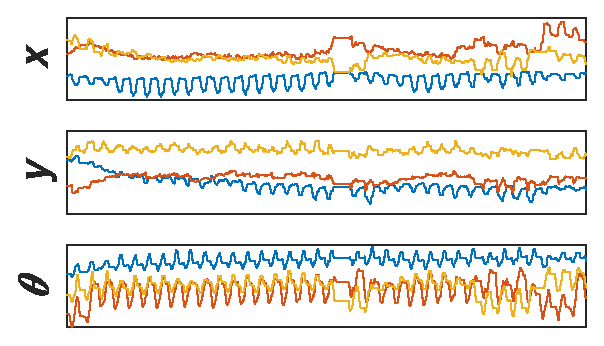
\includegraphics[width=1\textwidth]{crdDat.eps}
\caption{Smarticle coordinates and angles as tracked from experiments \label{fig:crdDat}}
	\end{subfigure}
	\begin{subfigure}[t]{0.4\textwidth}
	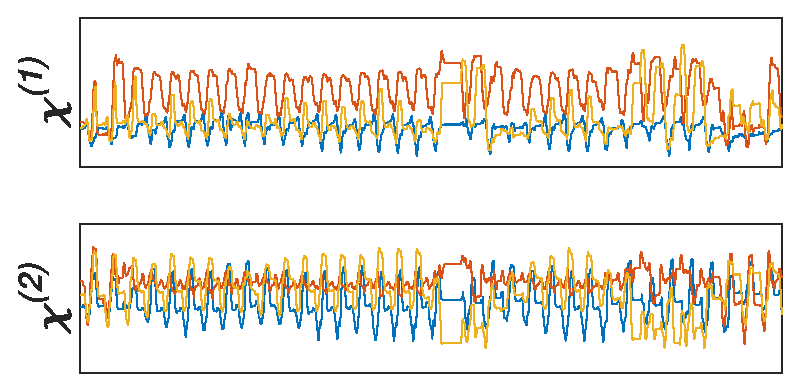
\includegraphics[width=1\textwidth]{relDat.eps}
	\caption{Rotationally invariant observables: c.o.m. coordinate as seen in the reference frame of each smarticle \label{fig:relDat}}
	\end{subfigure}
	\begin{subfigure}[t]{0.4\textwidth}
	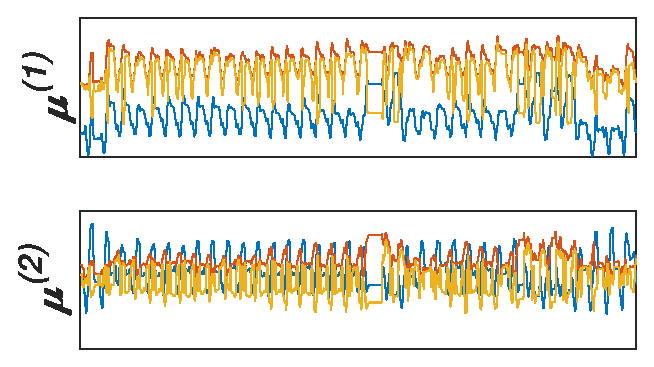
\includegraphics[width=1\textwidth]{piDat.eps}
	\caption{Permutation invariant observables: first 3 moments of the distributions in \ref{fig:relDat} \label{fig:piDat}}
	\end{subfigure}
	\begin{subfigure}[t]{0.5\textwidth}
	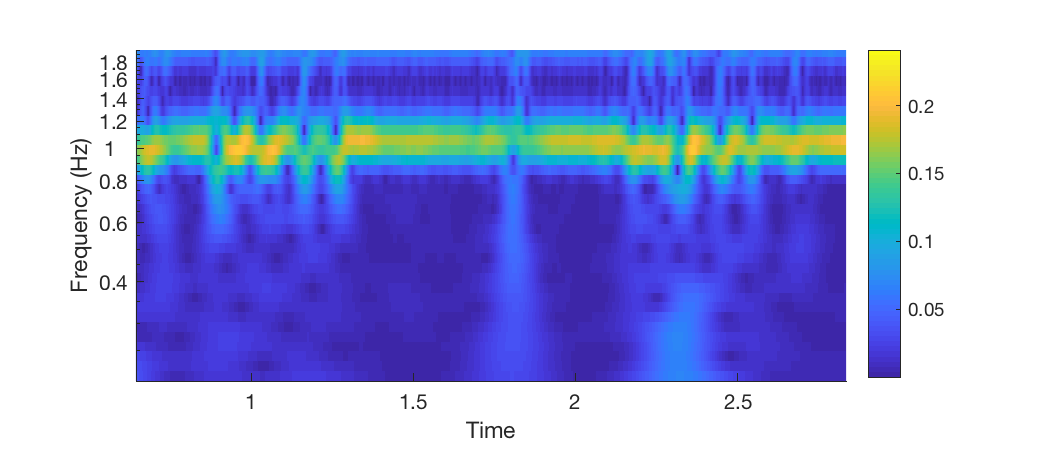
\includegraphics[width=1\textwidth]{wavelet.eps}
	\caption{Wavelet transform of one of the curves in \ref{fig:piDat}. We choose the values along the bright line for our feature vector. \label{fig:wavelet}}
	\end{subfigure}

	\caption{Data processing steps} \label{fig:1}
\end{figure}

\subsection{Modding out symmetries}
We begin by constructing functions of the raw data that are invariant under the symmetries we mentioned, but still sensitive to the information we may care about. The two symmetries are global rotations and permutation. To take care of the first, we find the coordinates of the c.o.m. $ \vec{X}= \frac{1}{3} \sum_i \vec{x}_i $ (note: permutation invariant) in the reference frame of each smarticle: $ \vec{\chi}_i \equiv \mathcal{R}(\theta_i) \cdot (\vec{X} - \vec{x}_i) $, where $ \mathcal{R}(\theta_i) $ is the rotation matrix for $ i $-th smarticle (fig \ref{fig:relDat}). Note that this is not a perfect choice: it is entirely invariant under c.o.m. translations (which is relevant, but we assume it to be small for a confined system), and smarticle orientation matters more the further it is from c.o.m. (so we must assume that their distance to c.o.m. stays relatively constant). We can often get away with such imperfect choices because we have so much overloaded data for the questions. 

Next, the permutation-invariant functions we choose are just the first three moments of the distribution of the three $ \{\chi_i\} $ at any fixed time. In order for these functions to have relatively similar sensitivity to changes in raw data, it helps to ensure that they have the same units -- by raising them to the appropriate fractional powers. I.e., $ \mu_1 = \frac{1}{3} \sum_i \chi_i $, $ \mu_2 = \sqrt{\frac{1}{3} \sum_i (\chi_i-\mu_1)^2} $, $ \mu_3 = \sqrt[3]{\frac{1}{3} \sum_i (\chi_i-\mu_1)^3} $ (fig. \ref{fig:piDat}). Note also that up to 3, these are the same as the cumulants -- which may be a better alternative for more smarticles.

\subsection{Capturing dynamics}
Now we can proceed to dealing with the fact that behaviors we are looking for are dynamic states, and thus depend on multiple time-points. We thus want to construct some feature vector that captures the dynamics. The simplest idea of simply stacking $ \mu_i $ at different time-points on top of each other is not obviously wrong, but will give a feature vector that is very sensitive to the noise. Instead, the dynamical features we are looking for are better captured by Fourier modes. Further, since the dynamical phase can change on the time-scale of a few arm oscillations, we don't want to transform the entire time-series, but instead consider a continuous wavelet transform of the data (fig. \ref{fig:wavelet}). This beautifully separates out behaviors on different time-scales, and we can choose our feature vector based on the time-scale(s) we most care about. The simplest choice here is to take the time-scale corresponding to one gait-period -- since most of the activity happens there. Again, this is throwing away lots of data, but since at the end we just care about some low-dimensional behavior space, we are still left with more than enough (including other time-scales had little effect). 

This way our feature vector consists of 6 complex numbers (3 moments for each dimension of the 2D $ \chi $ vector). We do care about relative phase of oscillation in the wavelet transform -- to keep this in the most unbiased way, we simply take the 36 possible differences between the 6 complex numbers, and then take their absolute value. While this makes the feature vector unnecessarily long, this is fine since we only care about the relative distances between these, and duplicate vector components will simply sum up.

\subsection{Dimensional reduction and clustering}
Now that we have our feature vector, we can dimensionally reduce or cluster the data. The former is, in a sense, a ``smoother,'' less dramatic operation, and thus turns out to produce more accurate results. We can understand this by realizing that in either case, the goal is to preserve pair-wise distances as best as possible, and this is much easier to accomplish if you allow points to be placed anywhere in the $ \mathbb{R}^2 $ plane, rather than in one of 5 discrete states. Curiously, clustering even works better when performed on dimensionally reduced, rather than original data. The other advantage of dimensionally reducing first is that this gives us more information about how the data is distributed, without imposing the assumption that it is well-clustered. 

\begin{figure}
\begin{subfigure} [t]{0.45\textwidth}
	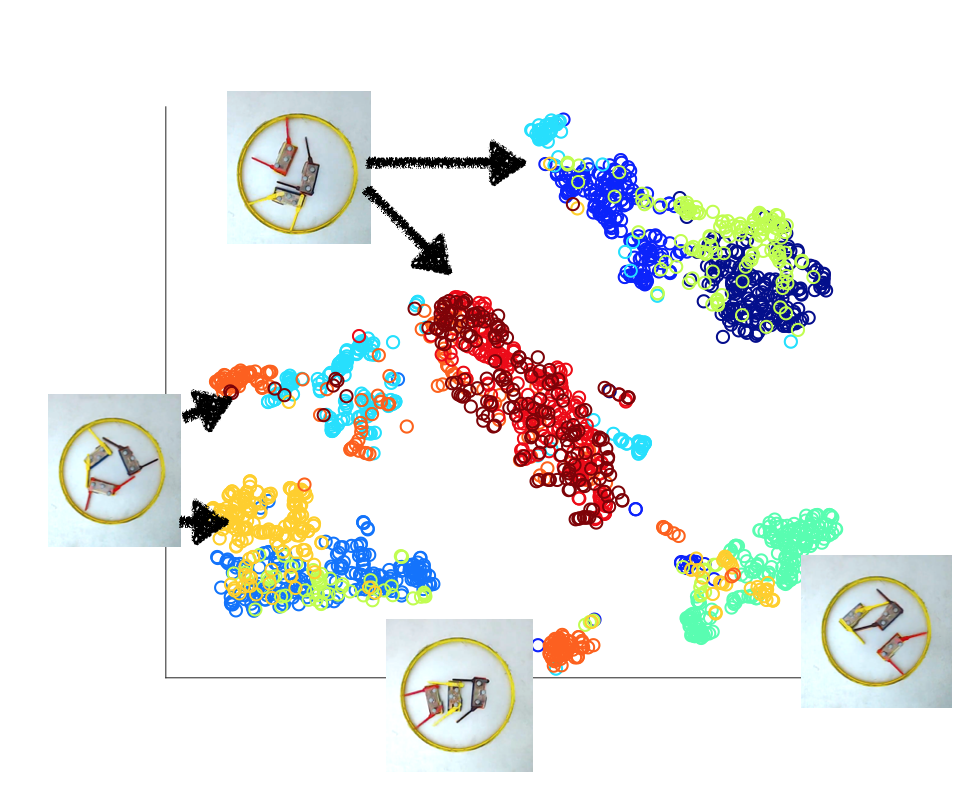
\includegraphics[width=\textwidth]{dimRedExp.png}
	\caption{Experiment \label{fig:dimRedExp}}
\end{subfigure}
\begin{subfigure} [t]{0.45\textwidth}
	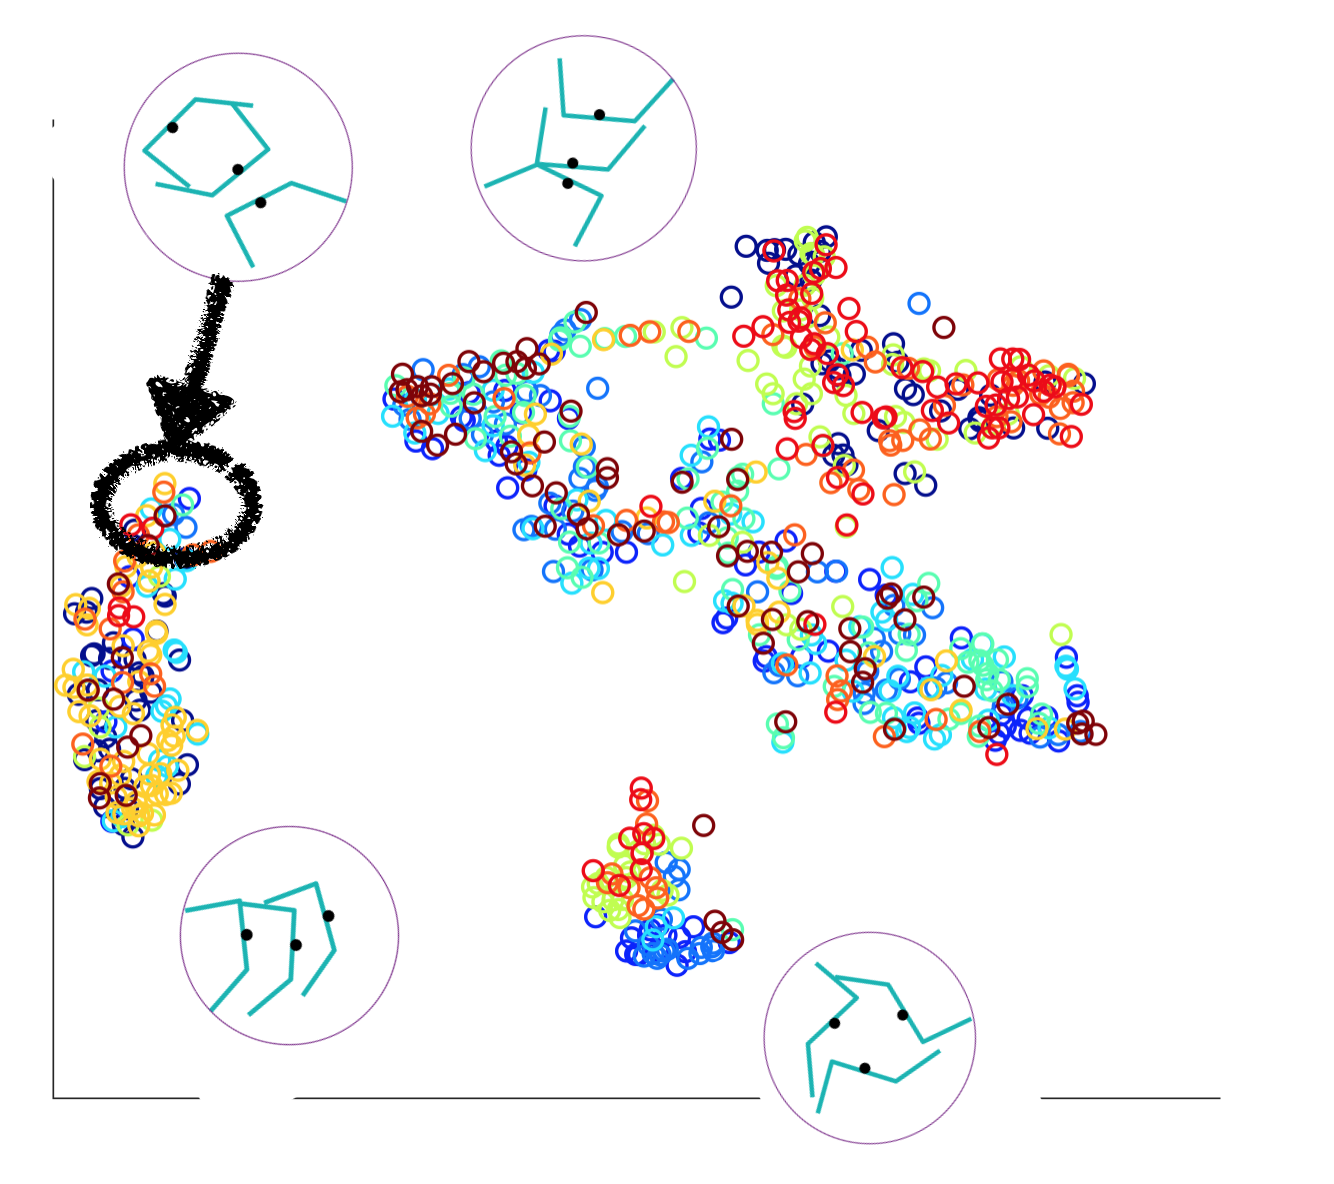
\includegraphics[width=\textwidth]{dimRedSim.png}
	\caption{Simulation \label{fig:dimRedSim}}
\end{subfigure}
\caption{Dimensionally reduced data. Insets show what sort of behavior each cluster corresponds to. Note that the cluster positions in the two plots are unrelated as the 2D embedding was done separately on two data sets. Color indicates different trials of the same experiment -- confirming that the behaviors are reproducible.}
\end{figure}

We use Matlab's built-in t-Distributed Stochastic Neighbor Embedding (tSNE) algorithm, which basically tries to embed the data in a 2D space preserving all the pair-wise distances as much as possible (fig. \ref{fig:dimRedExp}). It has the effect of largely preserving, or even highlighting, clusters in the original data, but also allows visualizing transitions between them and other hierarchical structure in the data. Note that the two pairs of clusters corresponding to the same pictures are chiral complements (the other two clusters correspond to non-chiral states). In section \ref{sec:dynPhaseTrans} below we will cluster this data and study the slow transition statistics between different dynamical phases.

\section{Simulation}
For easier exploration of hypothesis space of this system, we have constructed a numerical simulation with the following algorithm. We approximate smarticles by three-segment lines (insets in fig. \ref{fig:dimRedSim}). At each time-step, the algorithm moves the arms slightly according to the chosen gait, and then iteratively cycles through smarticle pairs in random order, checking for collisions, and moving one in each pair slightly according to the net interaction force. If there are multiple points of contact for a given pair, the move is a translation in the direction of the total force, otherwise, it is a rotation about a pivot point chosen so as to balance the forces and torques. Choosing which in the pair moves is random, weighted by their relative friction coefficients (as motivated by difficulty of predicting static friction). Note that since a move can create new collisions with other smarticles, it is important to take small steps and iterate. The algorithm continues looping through pairs until all collisions are resolved, then proceeding to the next time-step. While this describes the core of the algorithm, there are a number of bells and whistles necessary to improve its stability and reliability:
\begin{itemize}
	\item  If two arms are near-parallel when they approach each other, they can pass through each other between ticks without ever intersecting. To prevent this, along with collision detection, we must explicitly test for this in each pair. We then store the order of the arms for a few ticks into the future to prevent them passing through each other in any of those times.
	\item In case a smarticle with small friction gets trapped between two others, it might rattle back and forth on each iteration of collision-resolution, with no net effect. To prevent this, we temporarily (until next tick) increase its friction each time a smarticle moves.
	\item In experiment, when resolving collision is too hard, the motor simply does not move (jams up). To allow for that possibility in simulation, we add an exit condition from the collision-resolving loop for when any one smarticle's temporary friction becomes very large - as this serves as a proxy for how much force a motor must provide. We then move the most colliding arm back to its last time-step, and try collision-resolving again. If everything resolves, that arm will then have a chance to catch up to where it needed to be over the following ticks.
	\item The resulting simulation turns out to be too clean, and so dynamical phases much more stable than in experiments. Since we want to study transition statistics, we must find ways to destabilize them. There are a number of places we can add noise: slight fluctuations of smarticles' positions and angles at each tick, or on each move, randomly varying gait amplitude, varying arm velocity, etc.
	\item The ring boundary is implemented similar to other smarticles, and collisions with it are resolved in the same loop. Alternatively, we can implement weakly confining potential to keep smarticles together in a more smooth way.
\end{itemize}

Even with all these additions, many differences remain between simulation and experiment: smarticles have non-zero thickness in experiments, friction forces between smarticles are often important on collisions, there are relief features on smarticle body not present in simulation that can get caught, and others. The consequence in this system is that while qualitative features can be recovered in the simulation, we don't generally expect quantitative agreement. We guess that these differences may become less important for ensembles with more smarticles -- as universal collective properties start to dominate. We also guess that analytical predictive power of least-rattling, or other similar techniques, could be more applicable in that regime.

\section{Quantifying rattling}
In order to apply the least-rattling framework to this system, we need to define the effective temperature for different slow time-scale states we observe. The tricky part here is to distinguish between integrable or periodic orbits, and chaotic unpredictable ones. The key distinction is that as we zoom out the time-axis, the displacement due to periodic orbits averages out to zero, while that due to noise grows with the square root of time-scaling (as per central limit theorem). This way stochastic behavior will have slow time-scale effects, while periodic behavior will not. 

In our least rattling paper, we had the expression for effective temperature as $ T_{eff}\propto \int_0^\inf ds\;\<F_i(t),F_j(t+s)\>_{s.s.} $, where $ F $ is the force on the slow variables, and the average is over the fast steady-state. This is difficult to apply in a case as here, where slow dynamics happen for the same variables as the fast. Instead, we first replace $ F $ with simply the configuration space coordinates themselves -- call them $ x $ -- and then look for metrics that will capture how much irregular motion these undergo. The other challenge is that in practice, we cannot truly sample the fast steady-state -- which would require many runs with different noise realizations. Instead, we want to be able to measure $ T_{eff} $ just from a single time-trace, appealing to ergodicity of the fast dynamics. This way, we replace the average by $ t $-integral, and get $ T_{eff} \propto \int_0^\inf ds\int dt\;x_i(t)\,x_j(t+s) $. One problem here is that slow dynamics are not infinitely slow, and so we only want to integrate over time-scales shorter than the ``slow'' ones. The other problem is that we must filter out any periodic fast behavior, leaving only the stochastic part. The first is easily solved with a high-pass filter. The second is generally more complex, and we could think about measures like the scaling of explored configuration space volume with time. While that may be accurate, it is difficult to compute in practice. An easier proxy comes from the observation that the power spectrum for white noise is constant for all frequencies, while for any fast periodic behavior, it will be sharply peaked in the UV. Thus, the random component of the fast dynamics should produce a flat background for the power spectrum, which is then easy to measure anywhere outside the peaks (and these are assumed to only be in the UV by time-scale separation). We thus arrive at our approximation for rattling: $ T_{eff} \propto \int_{\epsilon}^{\Lambda} d\omega\; x_i(\omega)\,x_j(-\omega)$, where the band-pass is given by the fast ($ \Lambda $) and slow ($ \epsilon $) time-scales. Note also that this can also be viewed as a Principle Component Analysis -type estimate of the explored configuration space volume.

In practice, since our data also has slow time-scale variation, it's easiest to compute this metric from the same wavelet transform we used to get our feature vectors (fig. \ref{fig:wavelet}) -- just averaging the amplitudes below the bright line. We can already see that every transition point between different behaviors is accompanied by a peak in that region, as we wanted. The result we get is a $ T_{eff} $ tensor, the full structure of which is important for slow dynamics. As a rough check, we can visualize its largest eigenvalue by plotting it on the color axis of the dimensionally reduced plot -- fig. \ref{fig:dimRed_colors}b. We see the expected structure where some behaviors always have lower rattling than others, and transition states around the boundaries of the clusters are high-rattling. Note also that the density of the cluster itself can be used as an indicator of rattling -- low rattling behaviors will be robust, yielding points closer to each other. This is consistent with the colors shown. \todo{I'm not sure if this is pretty much a tautology or a potential least-rattling prediction.}
% (though this is mostly tautological, so serves merely as a sanity check of our different algorithms).

\begin{figure*}
	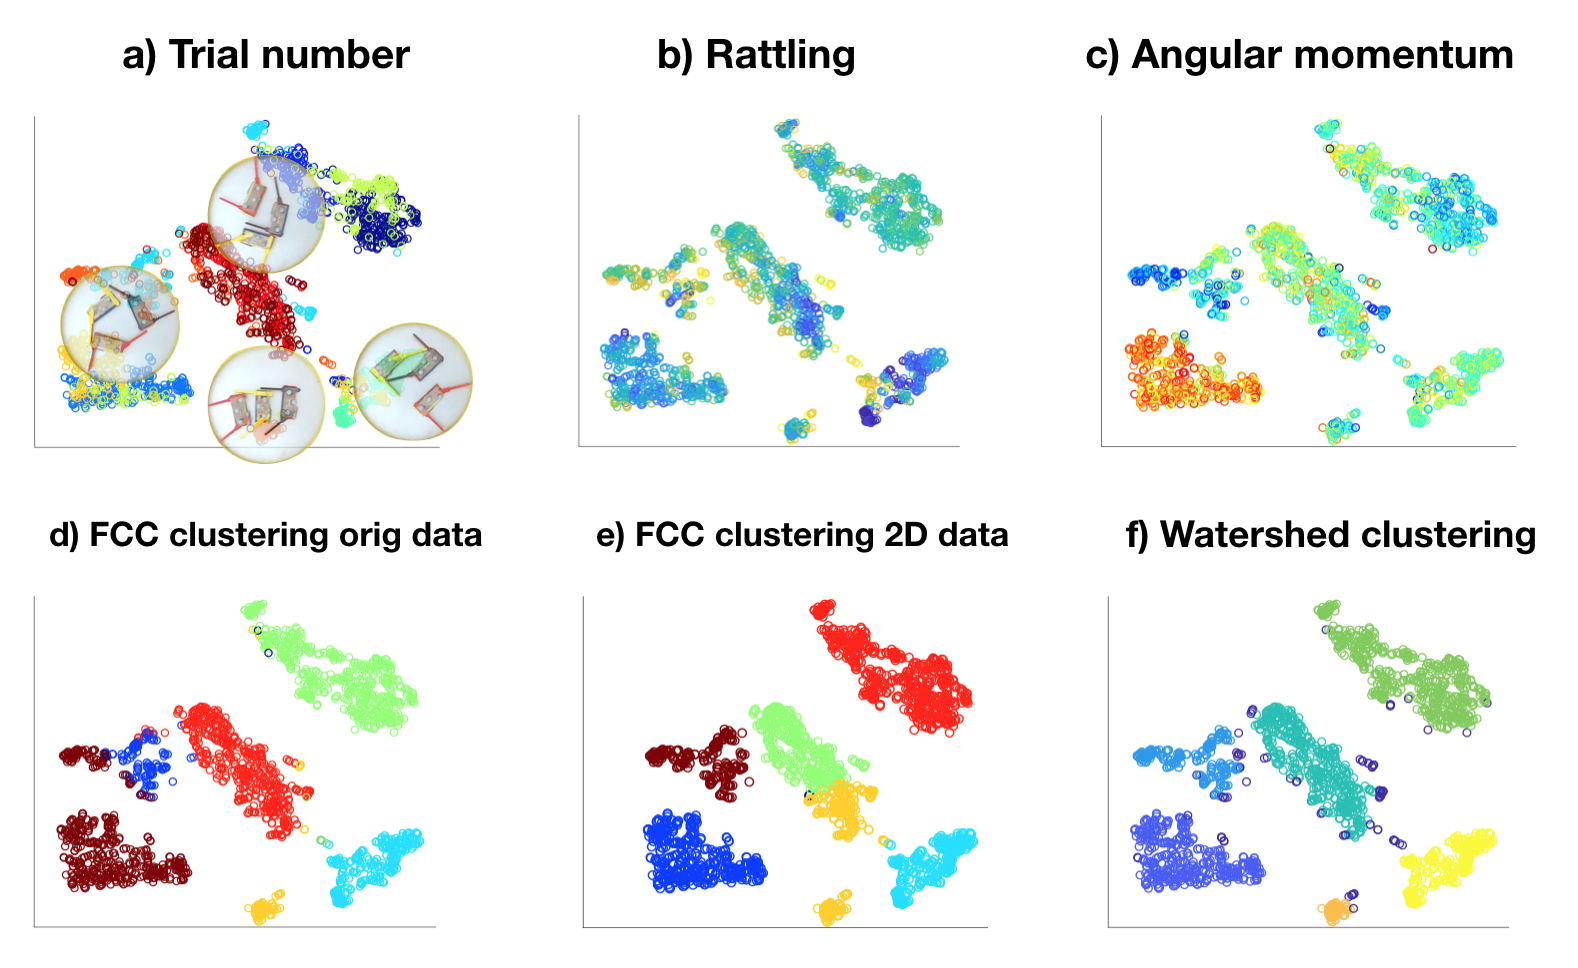
\includegraphics[width=\textwidth]{colorsExp.png}
	\caption{Different properties shown on the dimensionally reduced data \label{fig:dimRed_colors}}
\end{figure*}


\section{Dynamical phase transitions} \label{sec:dynPhaseTrans}

While dimensionally-reduced data visualization is informative about properties of different behaviors and relations between them in ways that clustering cannot be, identifying a discrete number of qualitatively distinct behaviors can be practical for making simple predictions on slow time-scale. For example, if we are interested in predicting the rate of global system rotation, knowing which discrete behavior it is in is mostly sufficient: plotting the values of global angular momentum in each state (fig. \ref{fig:dimRed_colors}c), we see that the two chirally opposite symmetric configurations account for most of the possible global rotation in the system. We can expect that other global system properties will similarly be mostly determined by the discrete behavior the system is in. 

The challenge of clustering behaviors is interesting. At first sight, it may seem to make more sense to run the clustering algorithm directly on the high-dimensional feature vectors. Using fuzzy c-means clustering (FCC) algorithm, and specifying 6 clusters, we show the resulting label assignments in fig. \ref{fig:dimRed_colors}d. We see that one of the groups that looks like a cluster in the dimensionally-reduced representation, is assigned to two different clusters by this algorithm. Checking the corresponding behaviors, we confirm that, as the low-dimensional plot shows, this cluster assignment is incorrect. We then proceed to running the FCC algorithm on the 2D data (fig. \ref{fig:dimRed_colors}e), and see that again, it mostly does well, but fails because it tries to make clusters roughly the same size. Inspired by the fact that visually these clusters are easy to identify, we instead use image-analysis, rather than the data itself, to get the clusters. We thus convert the plot to bitmap, apply Gaussian blur filter to it, binarize the image based on some threshold intensity, and then apply watershed analysis to the resulting binary. The clustering we get is precisely what we wanted (fig. \ref{fig:dimRed_colors}f), and does not require specifying the number of clusters by hand.

To get decent statistics on the transition probabilities between these 6 clusters, we need to observe at least $ \Ord{10} $ transition events for each of the 36 possible transitions. In experiment, we observe, on average, one transition every 3 minutes, thus requiring roughly 1000 minutes (~17 hours) worth of data. Moreover, we want to compare these transition graphs for slightly different experimental setups. Thus, studying this in experiments is hard -- which is why we built the simulation, where it is much easier to collect good statistics. Figure \ref{fig:transGraph} shows the dimensionally reduced simulation data, clustered using watershed analysis, and overlayed with the graph of transition probabilities (edge weights are $ \pi_{i\rightarrow j} =p(j|i) $).

\begin{figure}
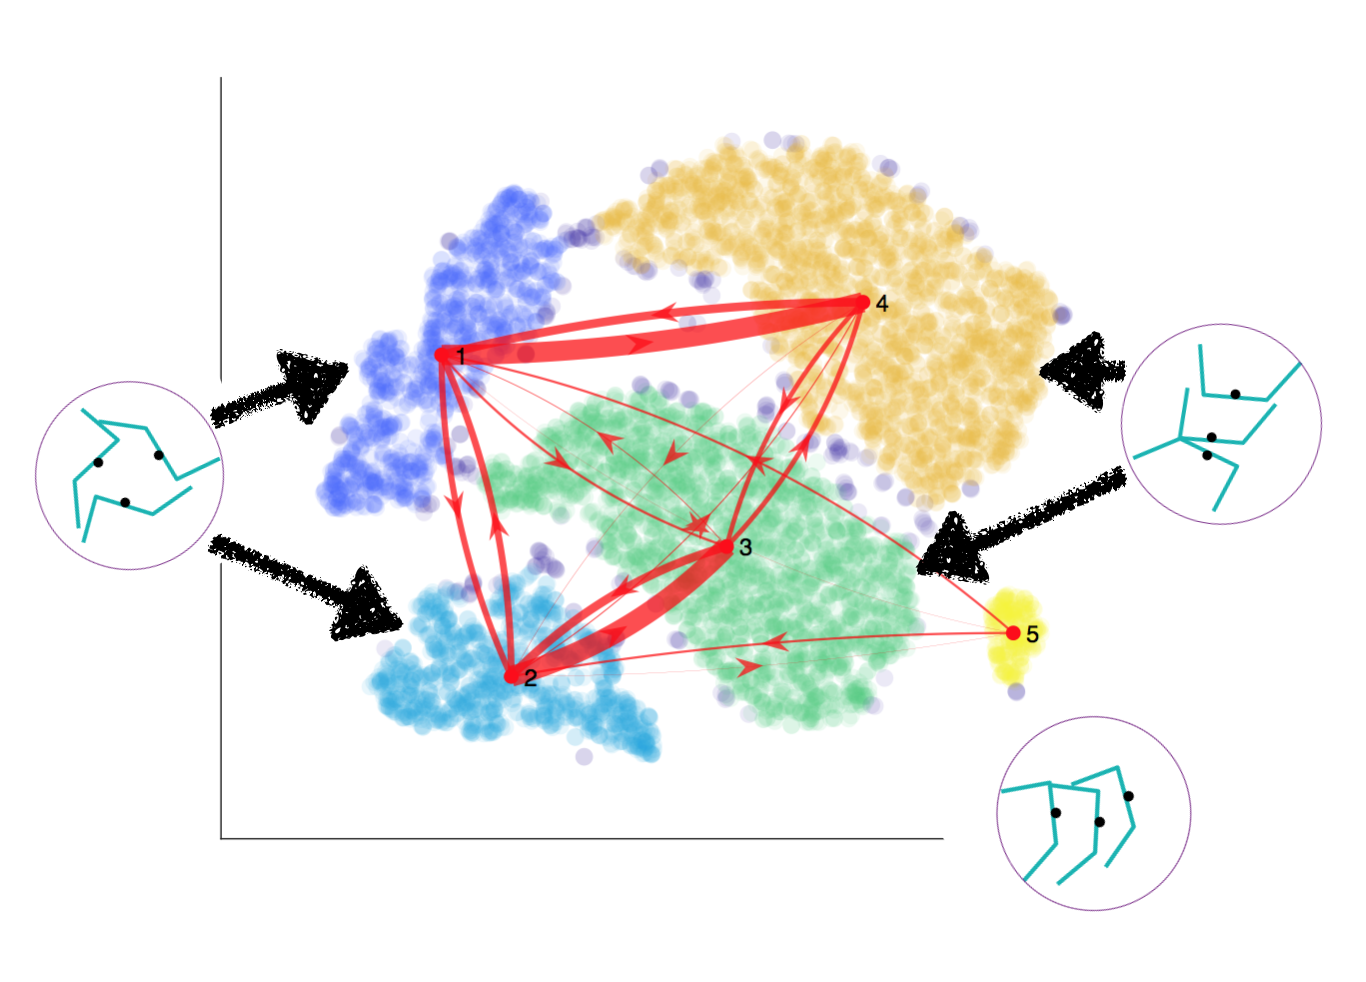
\includegraphics[width=0.5\textwidth]{transGraph.png}
\caption{Graph showing transition probabilities between regular states \label{fig:transGraph}}
\end{figure}

We can then play more with this graph and, for example, measure how much detailed balance breaking it shows. We can also used this graph to predict slow-time behavior of the system. For this, one important check we must first do is to see if the dynamics on this graph are Markovian, or if there is some memory of what the previous state was that is retained (this check was don't ion Gordon's paper - use their analysis).

%\nocite{*}
\bibliographystyle{unsrt}
\bibliography{/Users/pchvykov/Documents/GoogleDrive/MIT/RESEARCH/_data/14654301E131WECPZ6ZSATT3H7YHJ7G6D2E8/default_files/non-equilibSM.bib}
%/Users/pchvykov/Documents/Git/kr_cart_paper/non-equilibSM.bib

\end{document}
